\documentclass[main]{subfiles}

\begin{document}
\begin{lect}{2019-10-30}
    \begin{Definition}
        \[\Omega \text{ --- область в } \CC \q (\text{св., откр.})\]
        \[f \text{ --- голоморфной (аналит., регулярной) в  } \Omega, \text{ если }
            f \q \CC \text{ --- дифф.} \q \forall  z \in \Omega\]
        \[f'(z) \in C(\Omega) \text{ (потом узнаем, что это условие лишнее)}\]
        \[f \text{ - голом. в } \Omega \rla f \in  H(\Omega)\]
        \[f \text{ - целая, если } f \in H(\CC)\]
        Формальные произв.
        \[\frac{\partial f}{\partial z}; \ \frac{\partial f}{\partial \overline{z}}\]
        \[\begin{cases}
                z = x + iy \\
                \overline{z} = x - iy
            \end{cases}\]
        \[\begin{matrix}
                x = \frac{z + \overline{z}}{2} \\
                y = \frac{z - \overline{z}}{2i}
            \end{matrix}\]
        \[\frac{\partial f}{\partial z} = \frac{\partial f}{\partial x} \cdot
            \frac{\partial x}{\partial z} + \frac{\partial f}{\partial y}
            \frac{\partial y}{\partial z} = \frac{1}{2}(\frac{\partial f}{\partial x} - i
            \frac{\partial f}{\partial y})\] %%%%%%TODO ПРоверить НА логичЕскую Ошибку!!
        \[\frac{\partial f}{\partial \overline{z}}
            = \frac{1}{2}(\frac{\partial f}{\partial x} +
            i\frac{\partial f}{\partial y})\]
    \end{Definition}

    \begin{Definition}[усл. К-Р \ в терминах формальных производных]
        \[u_x' = v_y'\]
        \[u'_y = -v_x'\]
        \[\begin{matrix}
                \frac{\partial f}{\partial x} = u'_x + iv_x' \\
                \frac{\partial f}{\partial y} = u'_y + iv'_y
            \end{matrix}\]
        \[2 \frac{\partial f}{\partial z} = \us{=0}{u'_x - v'_y} + i(\us{=0}{
                v'_x + u'_y}) = 0\]
        \[\text{Усл К-Р } \rla \frac{\partial f}{\partial \overline{z}} = 0\]
    \end{Definition}

    \begin{Definition}[обратное отображение и якобиан]
        \[f \in H(G), \q \text{предп } z_0 \in \Omega \qq f'(z_0) \neq 0\]
        \[f = u + iv\]
        \begin{figure}[H]
            \centering
            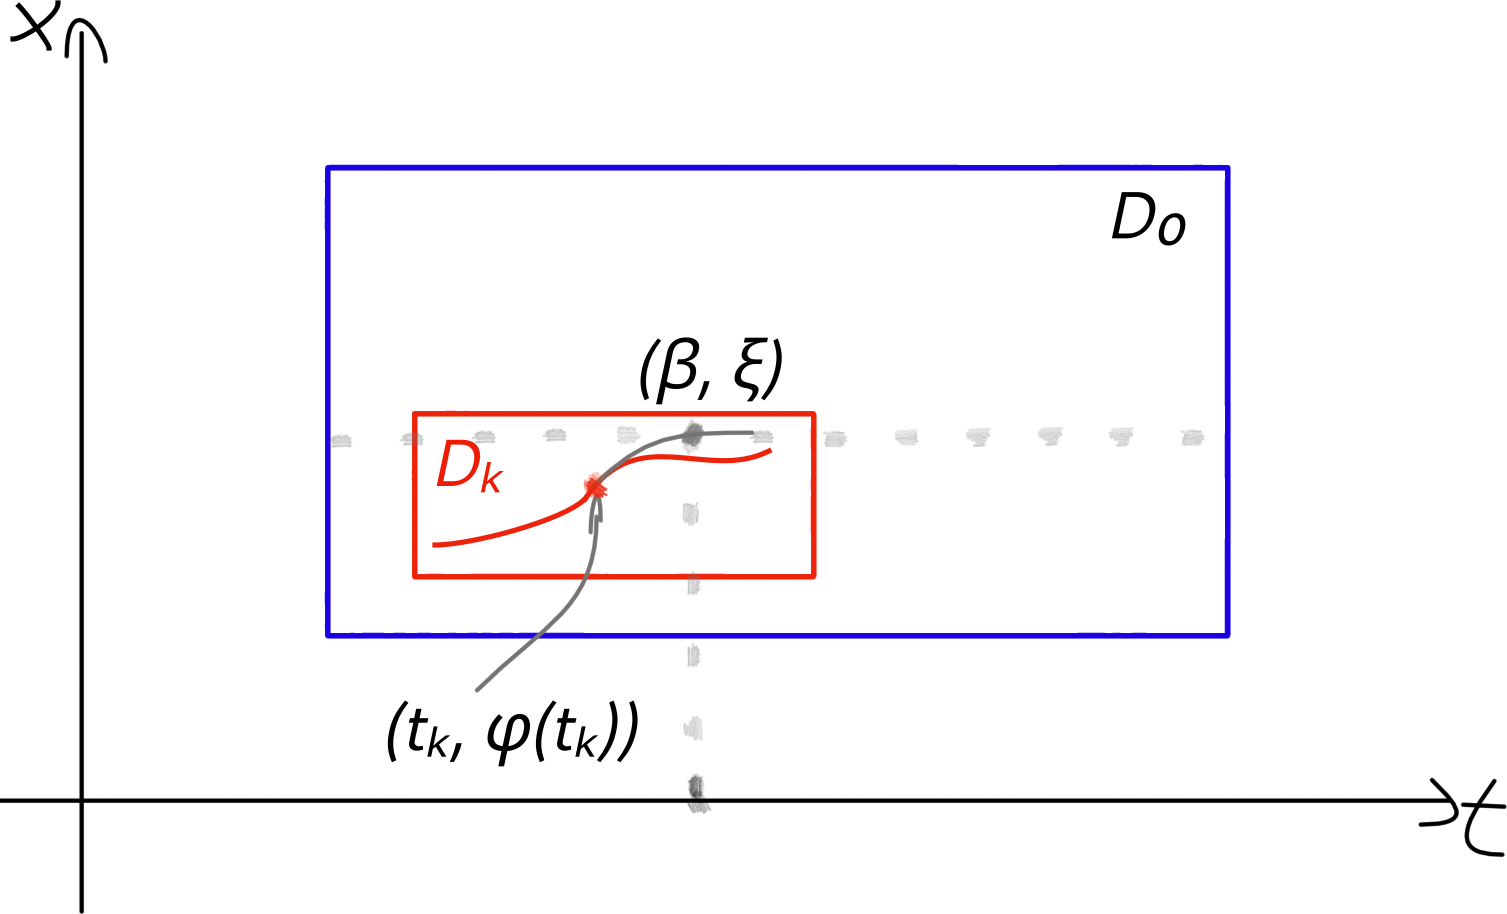
\includegraphics[width=2.5cm]{10_1}
        \end{figure}
        \[\text{Рассм. как отобр. } \Omega \subset \R^2\]
        \[(x, y) \os{f}{\to } (u, v)\]
        \[J_f = \begin{pmatrix}
                u'_x & u'_y \\
                v'_x & v'_y
            \end{pmatrix}\]
        \[\det(J_f) = u'_x v'_y - u'_y v'_x = (u'_x)^2 + (v'_x)^2 = \abs{f'}^2\]
        \[\det J_f = \abs{f'}^2\]
        \[\text{Если } f'(z_0) \neq 0 \Ra \det J_f(z_0) \neq 0\]
        \[\text{Можно применить теорему об обратном отобр.}\]
    \end{Definition}

    \subsection{Теорема (условия, достаточные для постоянства аналитической функции)}

    \begin{Theorem}
        \[f \in H(\Omega) \q z_0 \in \Omega \q f'(z_0) \neq 0\]
        \[\text{Тогда } \exists U \subset \Omega \q U \text{ --- откр. } \q z_0 \in U:\]
        \[f\big|_U \text{ --- инъекция } f(U) = V \text{ --- откр.}\]
        \[\text{И обр. отобр. } f^{-1}  : V \to U \text{ --- голоморф.}\]
        \[\text{Причем } (f^{-1})'(f(z)) = \frac{1}{f'(z)}\]
        \[(f^{-1} )(\omega) = \frac{1}{f'(f^{-1}(\omega))}\]
        \hline
        \[\exists U, V : \q f : U \to  \us{\text{откр}}{V} \text{ --- биекция из т. об обратном отобр.}\]
        Надо проверить диф-сть $f^{-1} $ в $g$
        \begin{figure}[H]
            \centering
            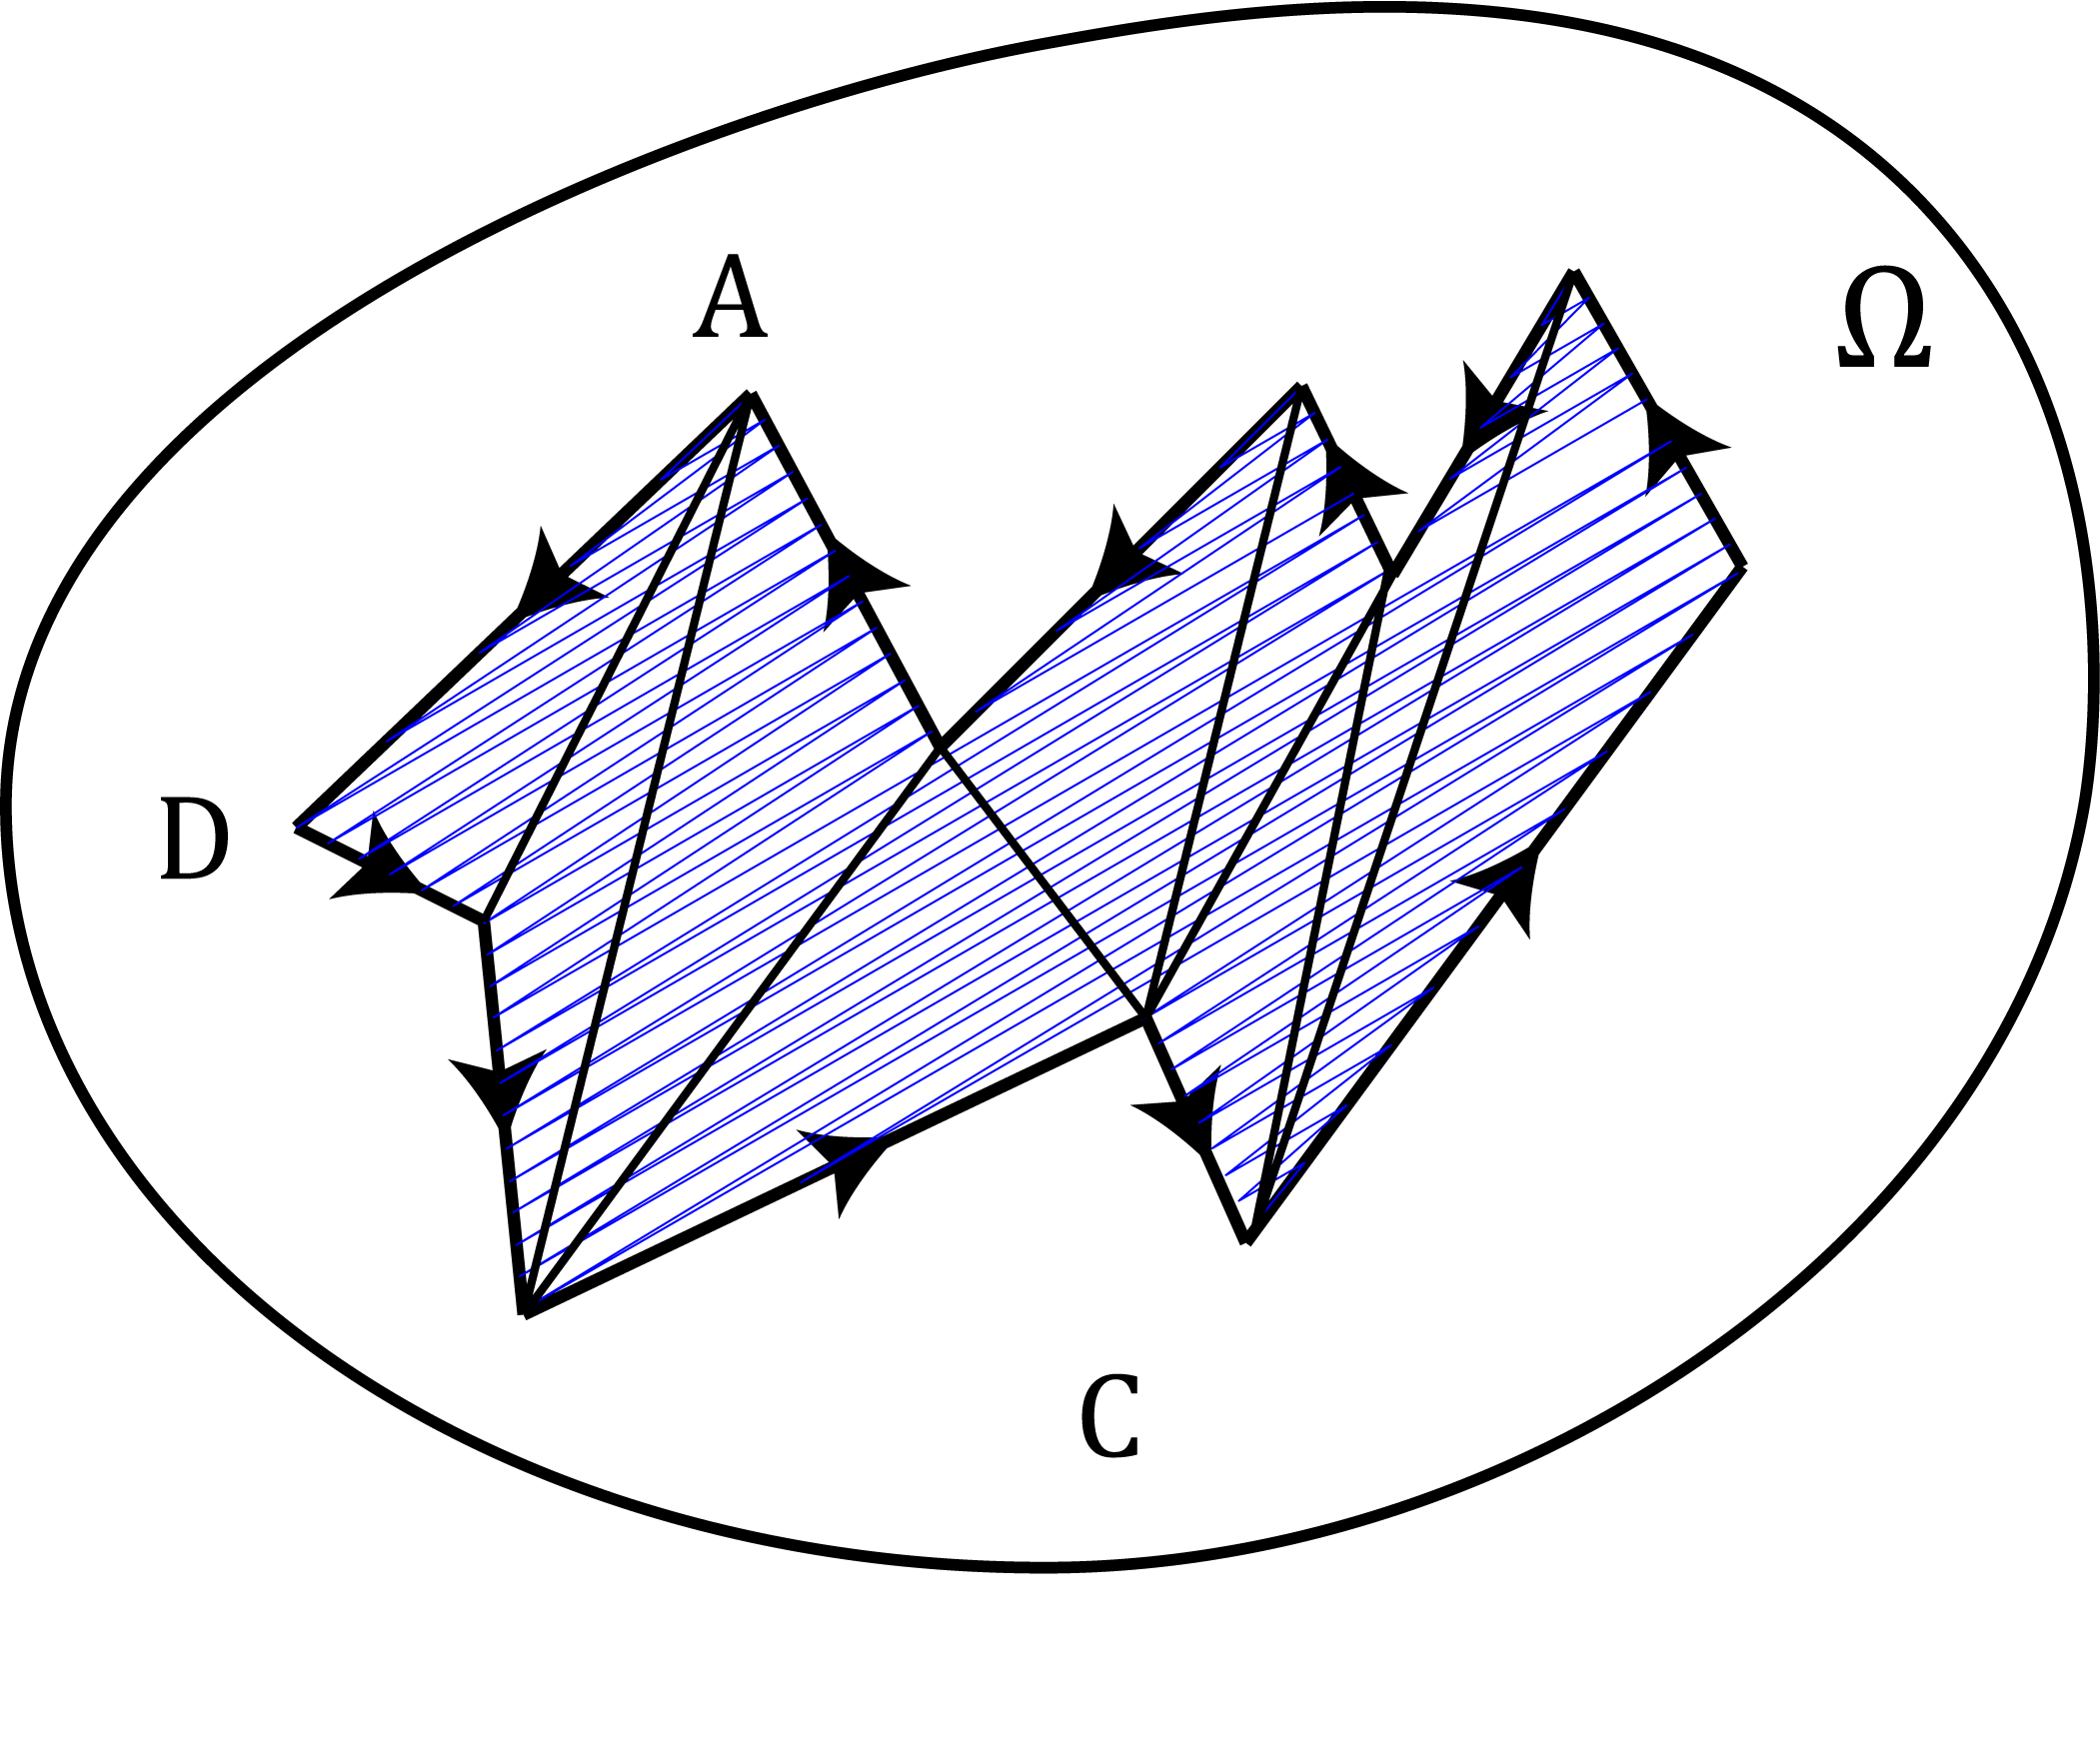
\includegraphics[width=8cm]{10_2}
        \end{figure}
        \[z_1 \in U\]
        \[\omega_1 = f(z_1)\]
        \[z \in U \q \omega = f(z)\]
        \[g = f^{-1}  : \ V \to U\]
        \[\lim_{\omega \to \omega_1} \frac{g(\omega) - g(\omega_1)}{\omega - \omega_1} =
            \lim_{\us{\Ra z \to z_1}{\omega \to \omega_1}} \frac{z - z_1}{f(z) - f(z_1)} = \]
        \[\lim_{z \to z_1} \frac{1}{\frac{f(z) - f(z_1)}{z - z_1}} =
            \frac{1}{f'(z_1)} = g'(\omega_1) = g'(f(z_1))\]
    \end{Theorem}

    \begin{Examples}
        \[1) \q z^n \in H(\CC) \text{ целая} \qq n \in \N\]
        \[P_n(z) \text{ --- мн-н --- целая ф-я}\]
        \[(z^n)' = nz^{n - 1} \in H(\CC) \subset C(\CC) \]
        \[\text{Рассмотрим } n > 1 \q z \neq 0 \Ra (z^n)' \neq 0\]
        \[\text{Выделим непрерывную ветвь } \sqrt[n]{z}\]
        \begin{figure}[H]
            \centering
            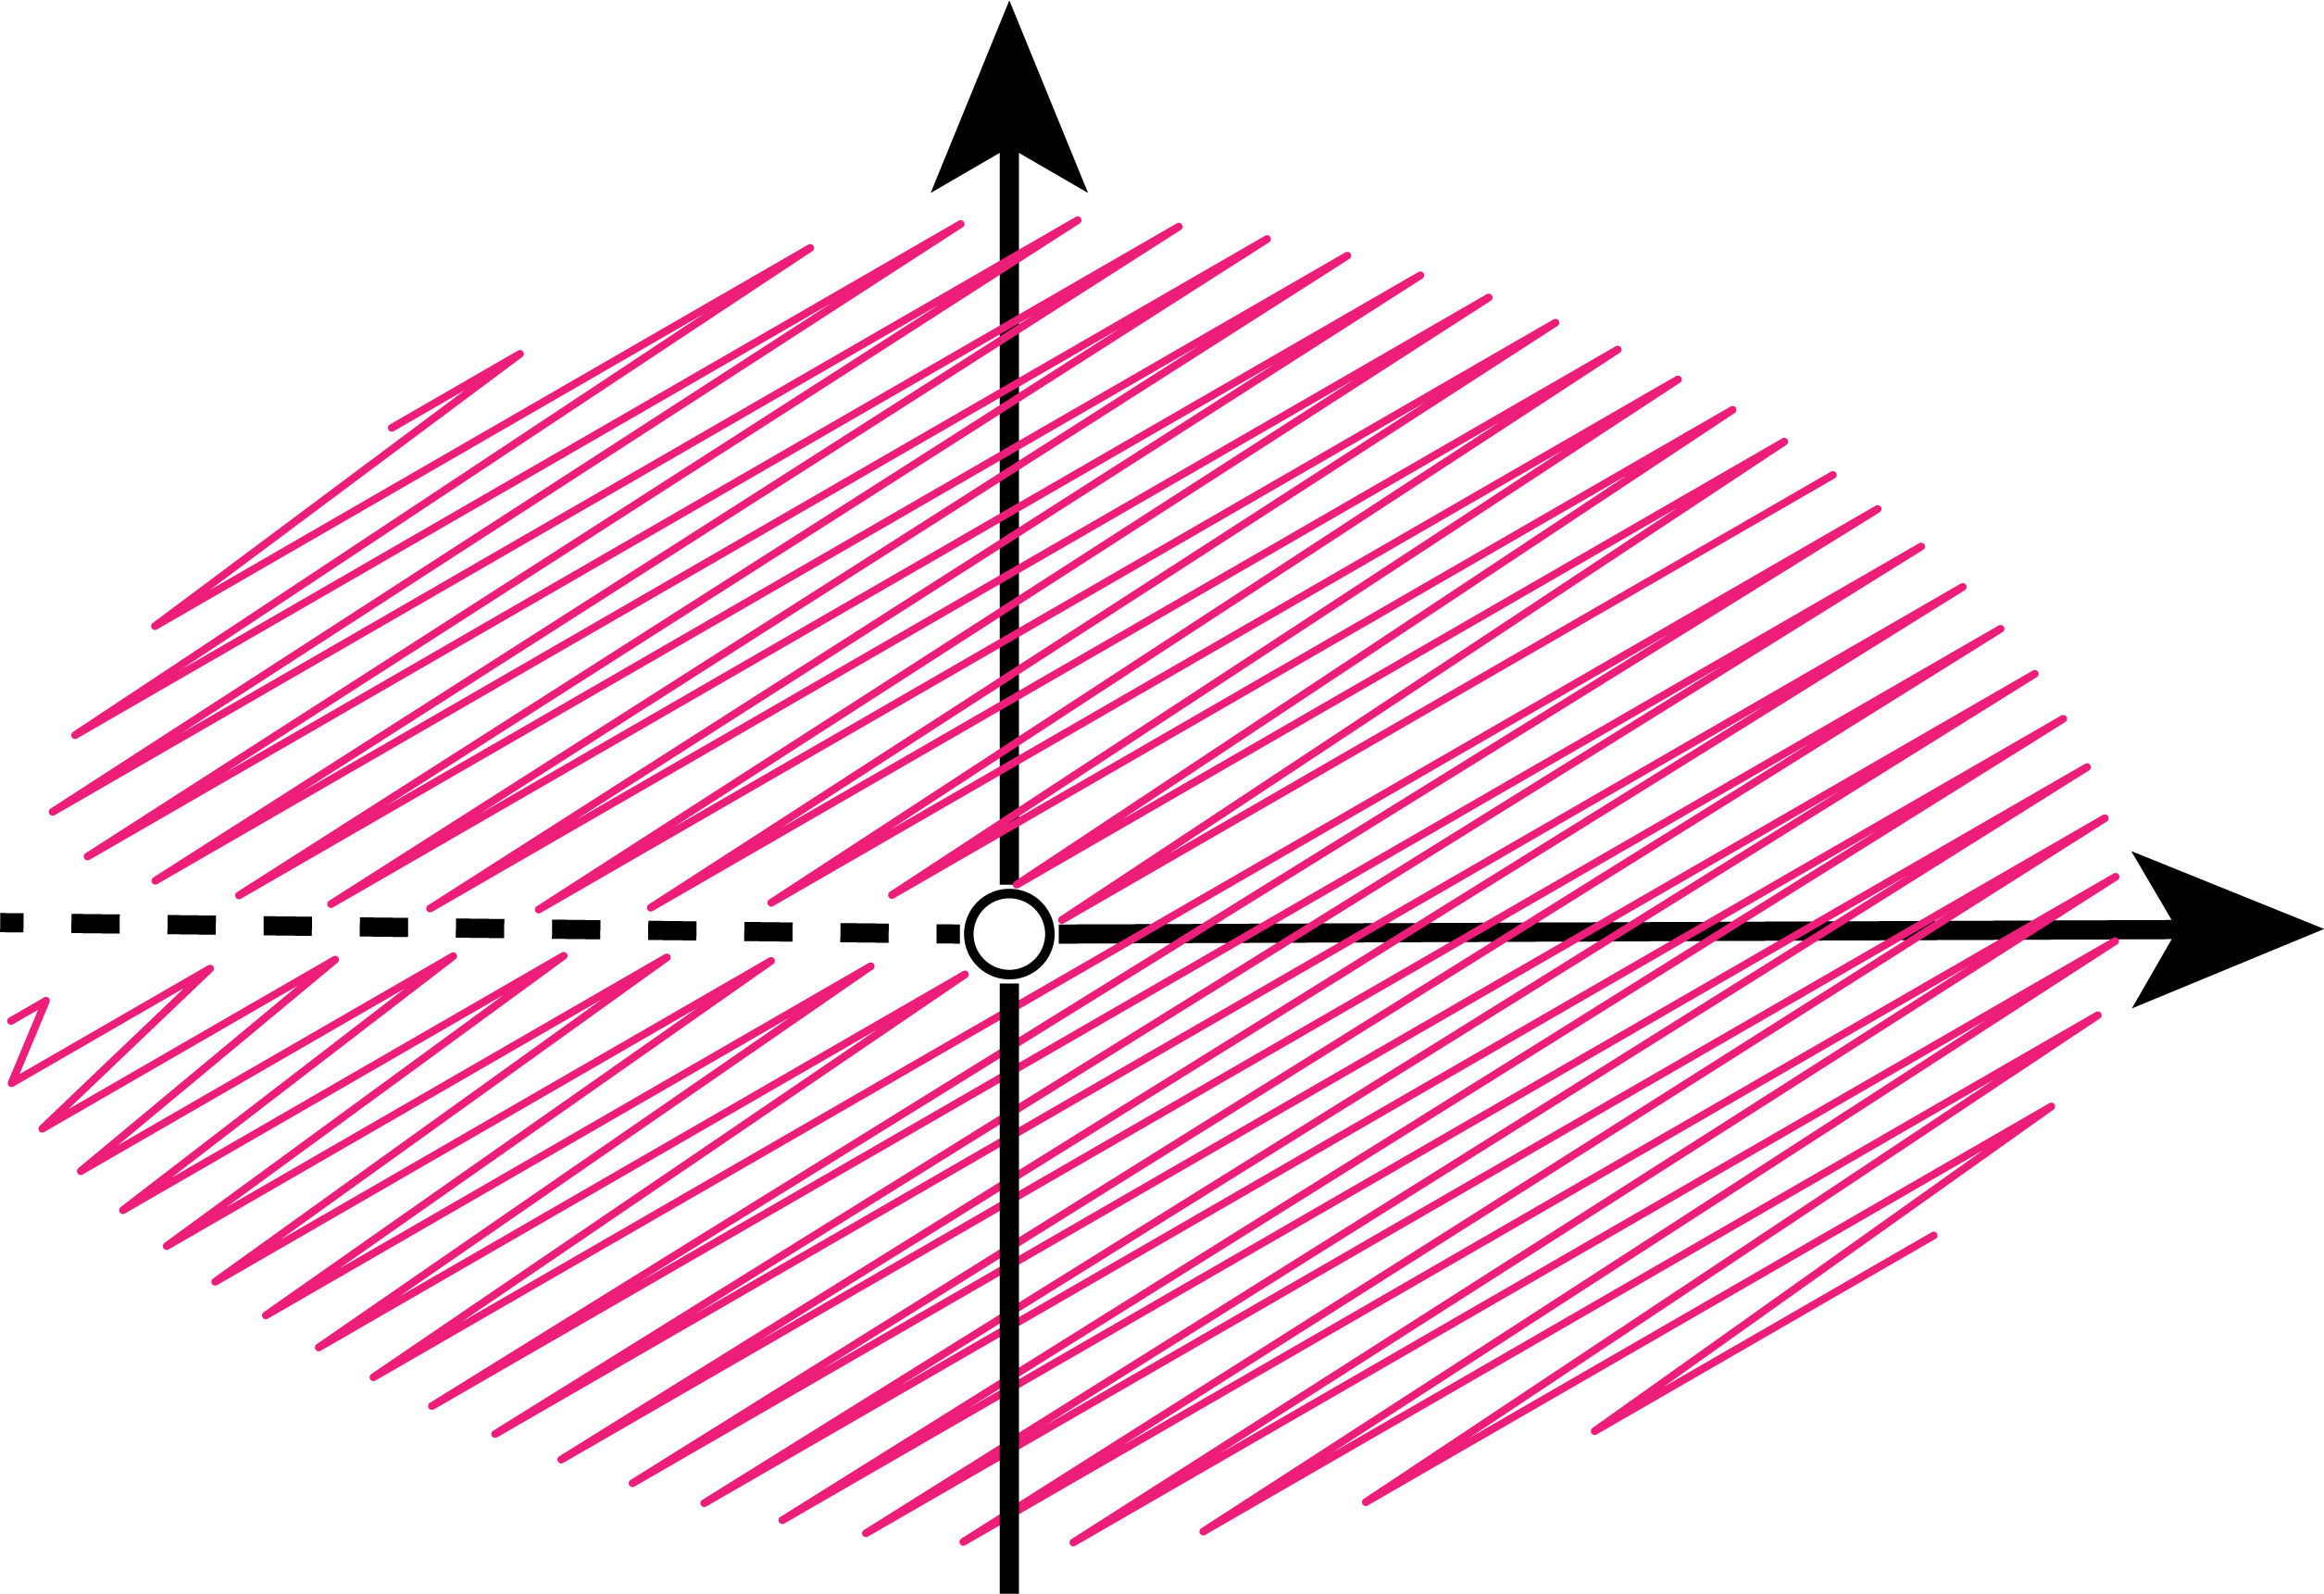
\includegraphics[width=5cm]{10_3}
        \end{figure}
        \[z^n = \omega\]
        \[(\sqrt[n]{z})' = \frac{1}{(z^n)'} = \frac{1}{nz^{n - 1} } =
            \frac{1}{n\omega^{1 - \frac{1}{n}}} = \frac{1}{n}\omega^{\frac{1}{n} - 1}\]
        \[2) \q f(z) = e^z = e^x(\cos y + i\sin y)\]
        \[u'_x = e^x \cos y = v'_y\]
        \[u'_y = -e^x \sin y = -v'_x\]
        \[f'(z) = \us{u'_x}{e^x \cos y} + i \us{u'_x}{e^x \sin y }= f(z)\]
        \[f'(z) \neq 0 \q \forall  z \in \CC\]
        Рассмотрим гл. ветвь лог-ма
        \[e^z = \omega\]
        \[\ln \omega = z \qq \varphi \in (-\pi; \pi)\]
        \[(e^z)' = f'(z) = e^z\]
        \[(\ln \omega)' = \frac{1}{f'(z)} = \frac{1}{e^z} = \frac{1}{\omega} \text{
                ; т.к. остальные ветви отличаются на константу}\]
    \end{Examples}

    \subsection{Интегрирование функции комплексного переменного по кривой. Свойства,  формула  Ньютона-Лейбница,  оценка  модуля  и  следствие  из
нее}

    \begin{Definition}[конформные отображения]\
        \begin{figure}[H]
            \centering
            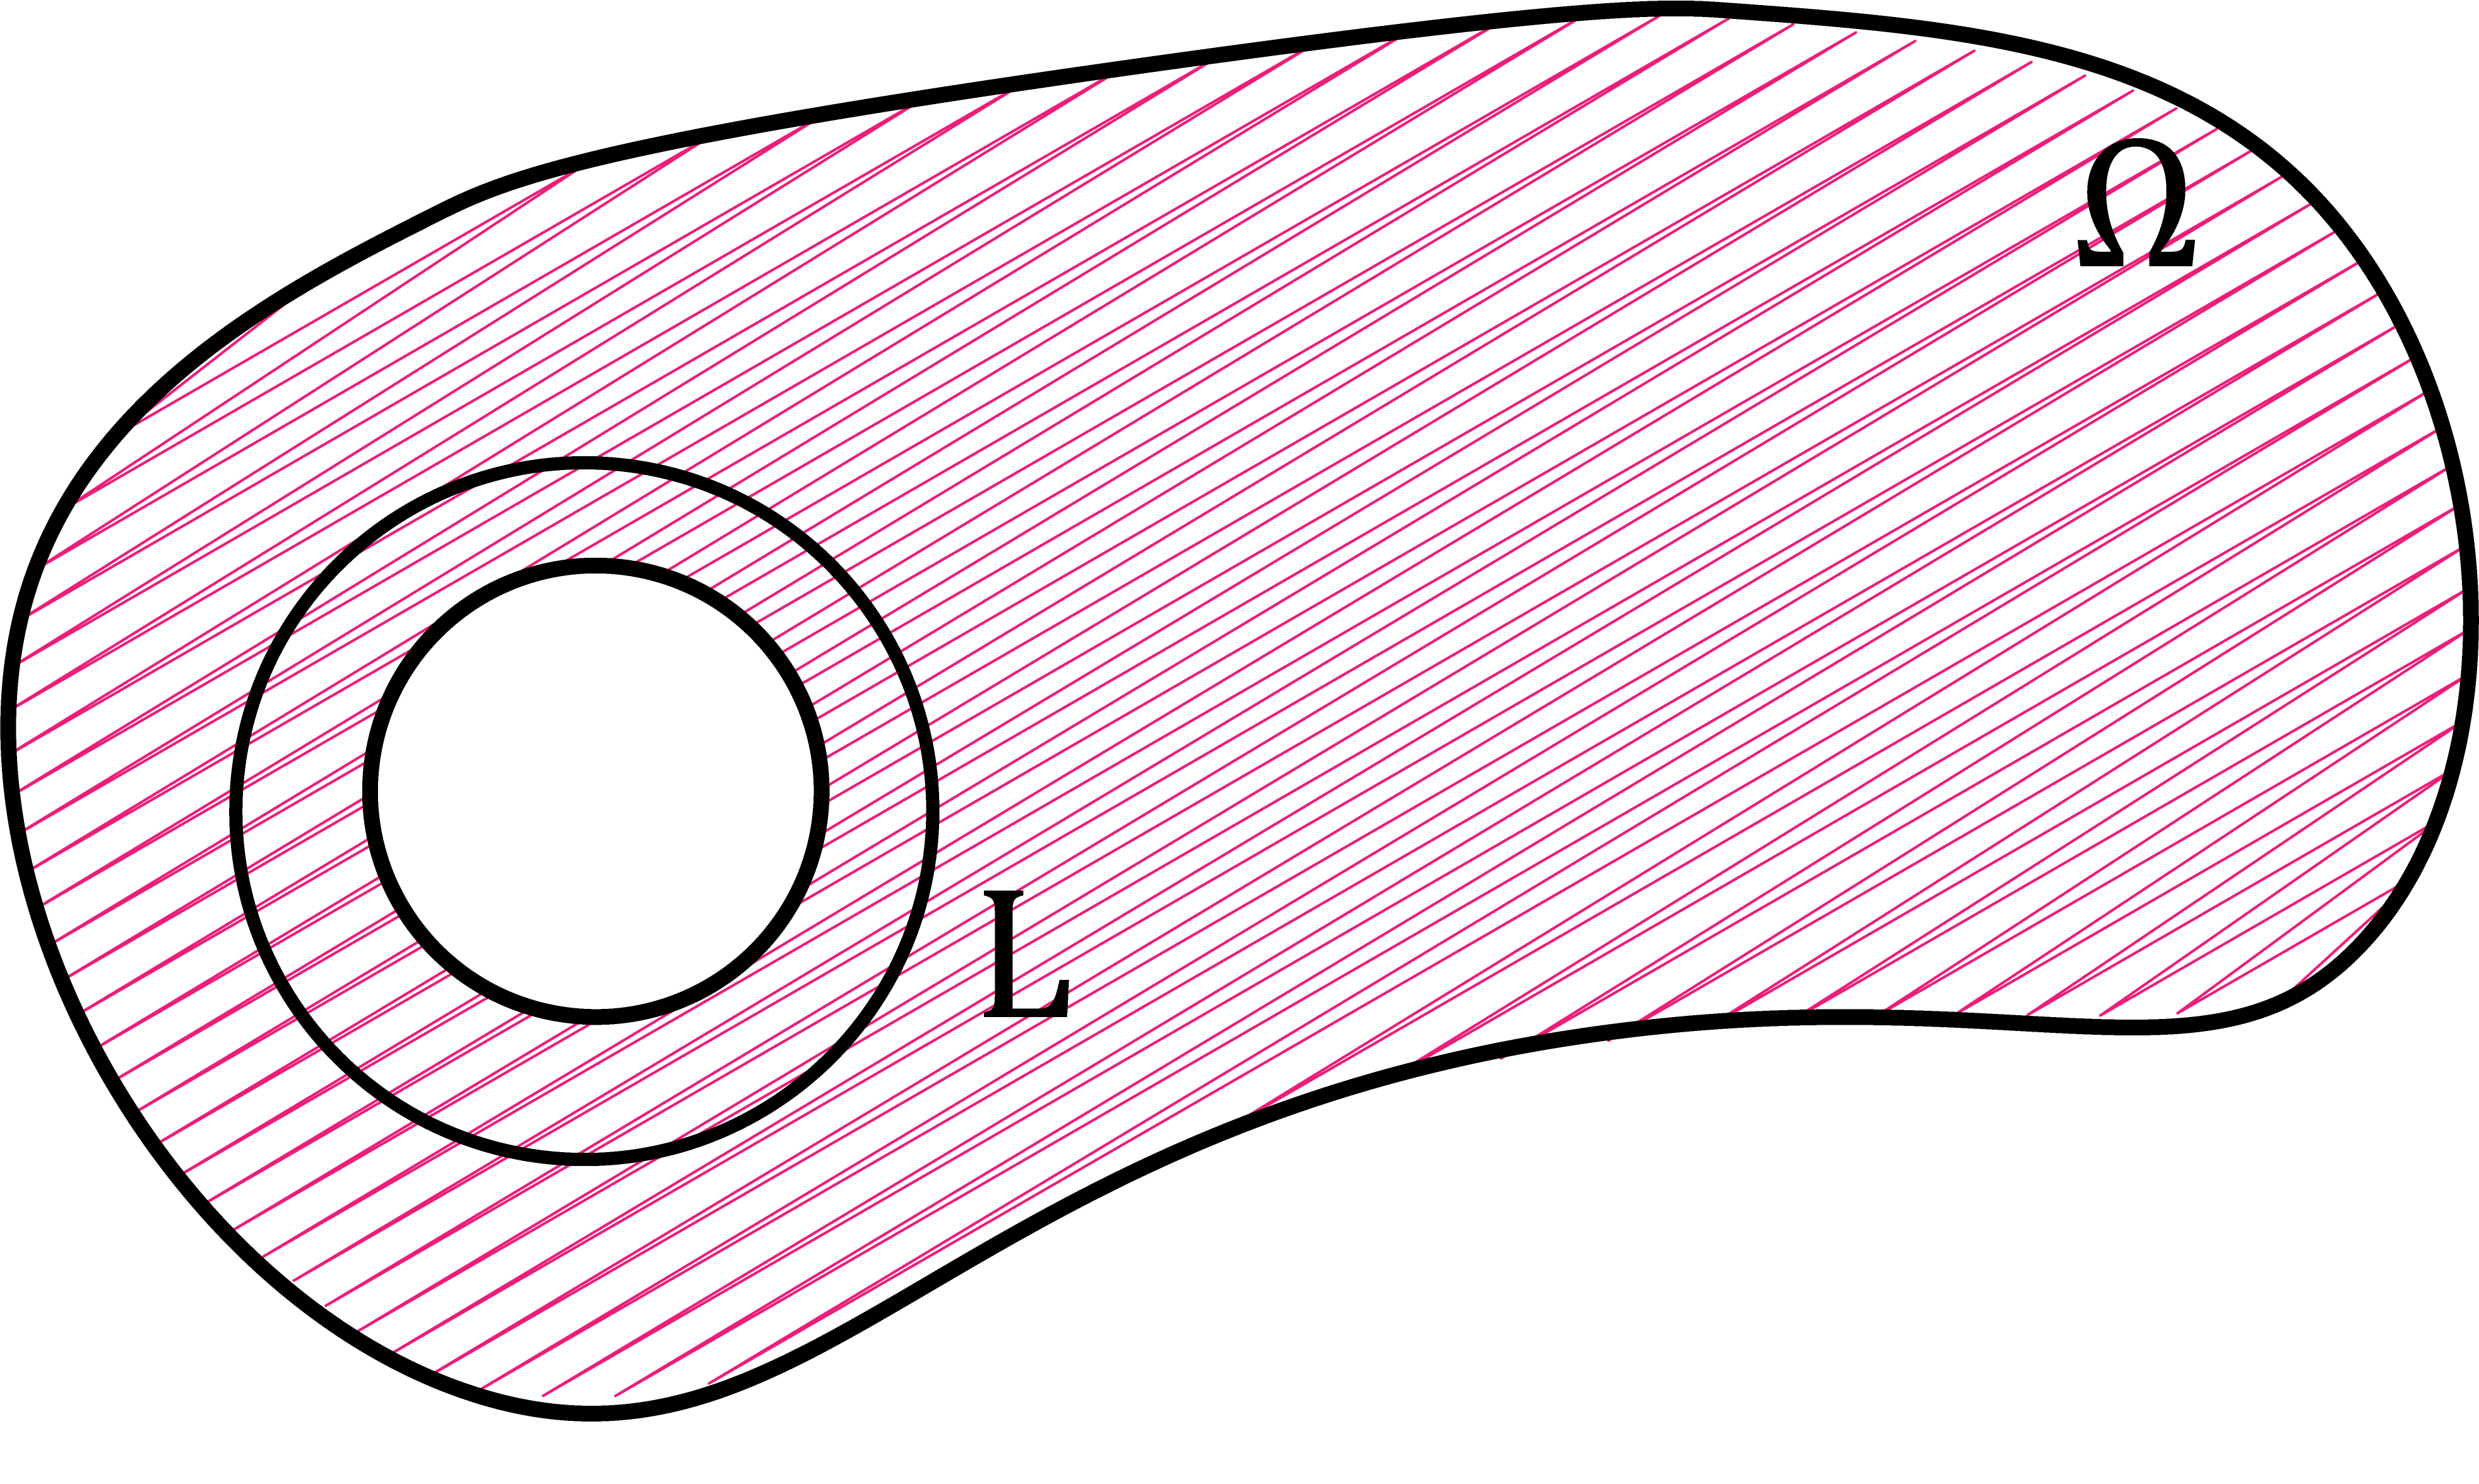
\includegraphics[width=3cm]{10_4}
        \end{figure}
        \[\gamma(t) = x(t) + iy(t) \qq 0 \leq t \leq 1 \qq \gamma \text{ --- гладкая кривая}\]
        \[\gamma'(t) = x'(t) + iy'(t)\]
        \[\gamma'(0) \text{ --- касат. вектор к } \gamma \text{ в т. } \gamma(0)\]
        \ul{Угол между кривыми} = угол между касат. в т. пересеч.
    \end{Definition}

    \begin{Theorem}
        \[\text{Пусть } \gamma(t) \text{ --- гладкая парам. кривой } \gamma\]
        \[z_0 = \gamma(0) \qq f \text{ --- аналитична в окрестности } z_0\]
        \[\text{Тогда касат. к } f(\gamma(t)) \text{ в т. } f(z_))\]
        \[(f \circ \gamma)'(0) = f'(z_0) \gamma'(0)\]
    \end{Theorem}

    \begin{Proof}
        \[\lim_{t \to 0}  \frac{(f(\gamma(t))) - f(\gamma(0))}{t} =
            \lim_{t \to 0} \underbracket{\frac{f(\gamma(t)) -
                    f(\gamma(0))}{\gamma(t) - \gamma(0)} }_{\to f'(z_0)}
            \underbracket{     \frac{\gamma(t) - \gamma(0)}{t}}_{\to \gamma'(0)} \]
    \end{Proof}

    \begin{Consequence}
        \[\text{Пусть } f \text{ --- аналит. в окр. т. } z_0\]
        \[\gamma, \widetilde{\gamma} \text{ кривые с гл. парам-ми}\]
        \[\gamma(0) =\widetilde{\gamma}(0) = z_0  \]
        \[\text{Если } f'(z_0) \neq 0 \text{, то угол (ориент.) между }
            \gamma \text{ и }
            \widetilde{\gamma} \text{ в т. } z_0\]
        \[\text{равен углу } f(\gamma) \text{ и } \widetilde{f(\gamma)} \text{ в т. }
            f(z_0)\]
        \begin{figure}[H]
            \centering
            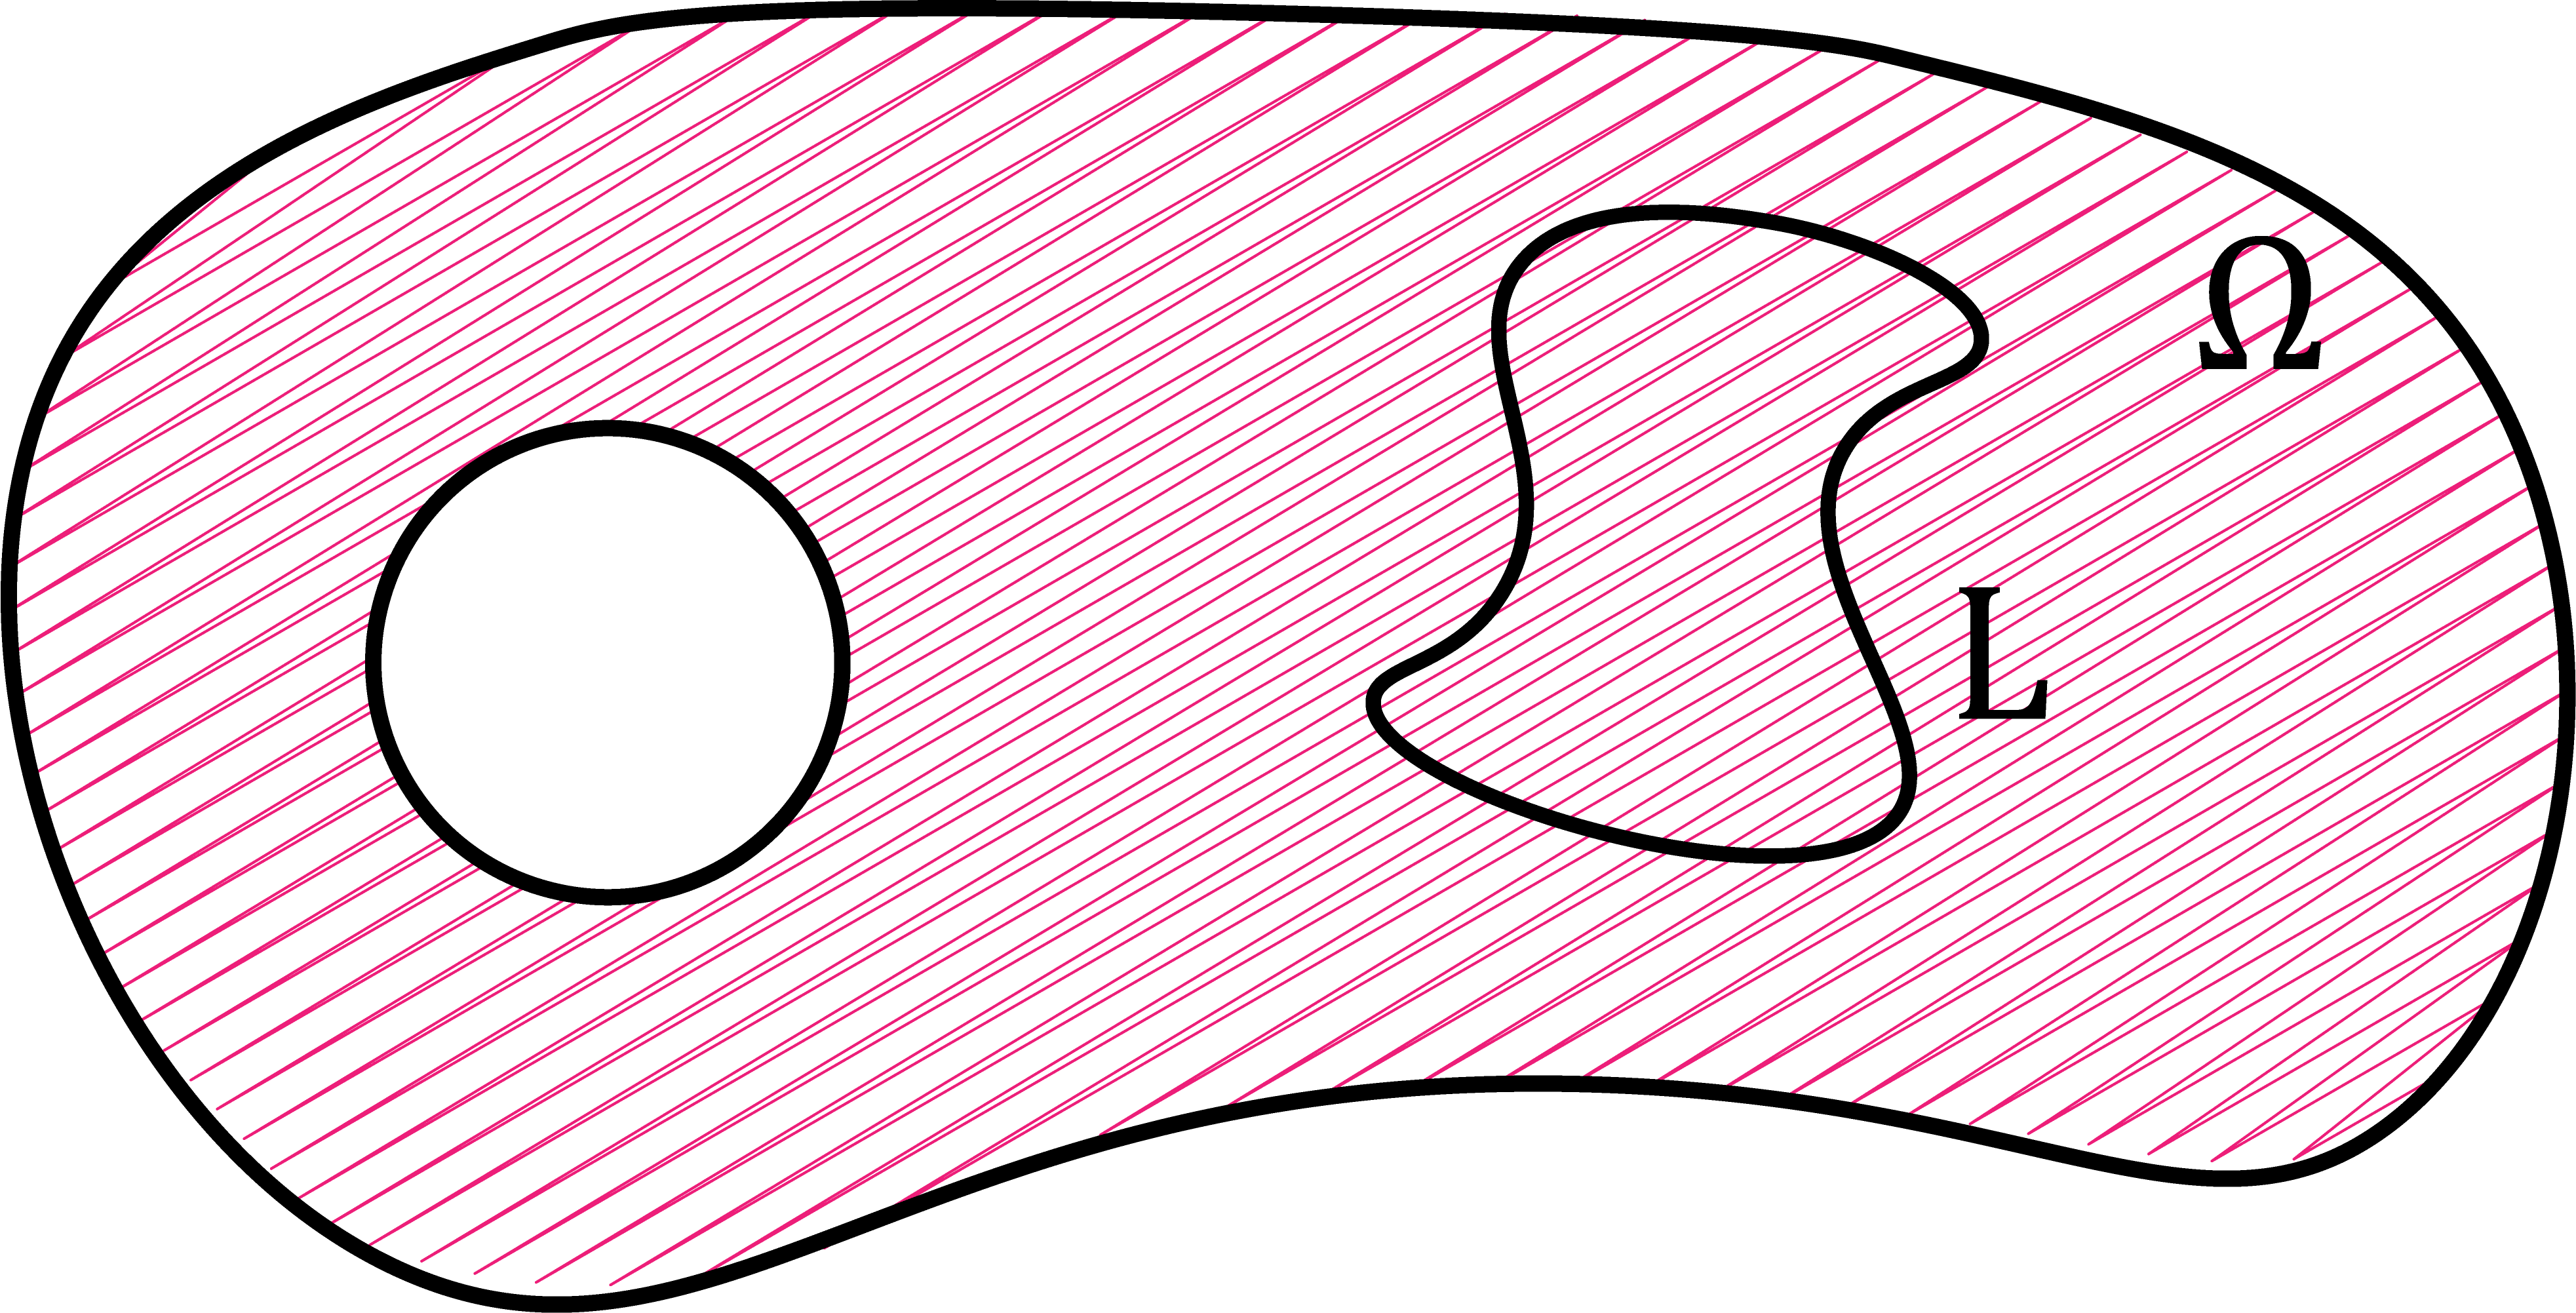
\includegraphics[width=9cm]{10_5}
        \end{figure}
        Такие отображения называются конформными
    \end{Consequence}

    \begin{Example}
        \[e^z; \q z^3 - \text{ конф. в } \CC \setminus \{0\}\]
    \end{Example}

    \begin{Definition}[интегралы]
        \[f : [a, b] \to  \CC \text{ - кус.-непр.}\]
        \[\int_a^b f(t)dt = \int_a^bu(t)dt + i\int_a^bv(t)dt\]
    \end{Definition}

    \begin{properties}
        \begin{enumerate}
            \item $\displaystyle  \abs{\int_a^bf(t)dt} \leq \int_a^b \abs{f(t)}dt$
                  \[\lambda = \frac{\int_a^bf(t)dt}{\abs{\int_a^bf(t)dt}} \text{, если }
                      \int_a^bf(t)dt \neq 0 \text{ (иначе очев.)}\]
                  \[\abs{\lambda} = 1\]
                  \[\abs{\int_a^bf(t)dt} = \lambda^{-1} \int_a^bf(t)dt =
                      \int_a^b\lambda^{-1} f(t)dt = \real \int_a^b\lambda^{-1} f(t)dt =  \]
                  \[=\int_a^b\real\lambda^{-1}f(t)dt \leq
                      \int_a^b \abs{\lambda^{-1}f(t) }dt = \int_a^b\abs{f(t)}dt\]
        \end{enumerate}
    \end{properties}

    \begin{Definition} [кусочно-гл. кривые в $\CC$]
        \[\gamma : I \to \CC \q \gamma' \text{ --- кус.-непр.} \qq \us{\text{откр.}}{I}
            \subset \R\]
        \[\text{Длина кривой } L(\gamma) = \int_{I} \abs{\gamma'(t)}dt\]
    \end{Definition}

    \begin{Definition}[криволин. инт-л от ф-ии $f$]
        \[\int_\gamma f(z)dz = \int_I f(\gamma(t)) \cdot \gamma'(t)dt\]
        \begin{figure}[H]
            \centering
            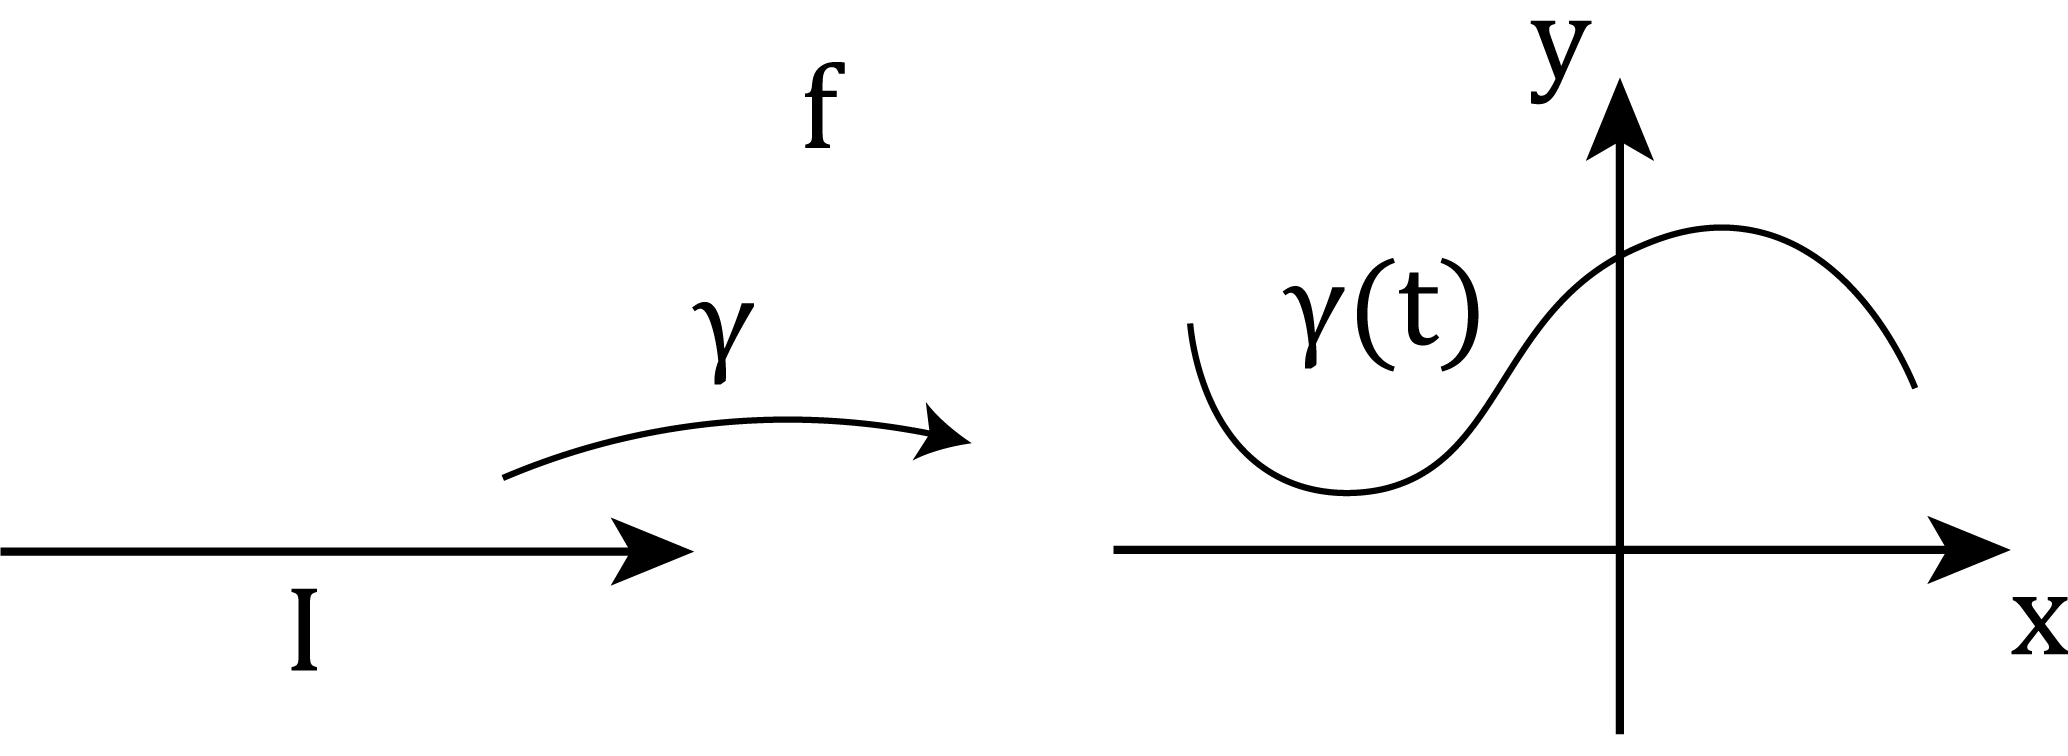
\includegraphics[width=7cm]{10_6}
        \end{figure}
    \end{Definition}

    \begin{properties}
        \begin{enumerate}
            \item Линейность
                  \[\int_\gamma (f + kg)(z)dz = \int_\gamma f(z)dz + k\int_\gamma g(z)dz \]
            \item Независимость от параметризации
                  \[\widetilde{\gamma} = \gamma \circ h \qq h'(t) > 0\]
                  \[\widetilde{\gamma} : [\widetilde{a}, \widetilde{b}] \to \CC\]
                  \[h : [\widetilde{a}, \widetilde{b}] \qq \gamma: [a, b] \to \CC\]
                  \[\int_{\widetilde{a}}^{\widetilde{b}} f(
                      \widetilde{\gamma}(t)) \cdot \widetilde{\gamma}'(t)dt =
                      \int_{\widetilde{a}}^{\widetilde{b}} f(\gamma(h(t))) \cdot \gamma'(h(t))
                      h'(t) dt = \bigg|^{h(t) = s}  \int_a^b f(\gamma(s))\gamma'(s)ds\]
            \item Изменение направления \\
                  $\gamma$ --- кривая с противоп. направлением
                  \[\int_\gamma f(z)dz = -\int_{-\gamma} f(z)dz \]
            \item Формула Ньютона-Лейбница \qq $\gamma: [a, b] \to \CC$
                  \[\int_\gamma f'(z) = \int_a^b f'(\gamma(t)) \cdot \gamma'(t)dt =
                      \int_a^b df(\gamma(t)) = \]
                  \[= \int_a^b du(\gamma(t)) + i\int_a^b dv(\gamma(t)) =
                      f(\gamma(b)) - f(\gamma(a))\]
        \end{enumerate}
    \end{properties}

    \begin{Example}[1]
        \[\int_\gamma (z - a)^n dz = \int_0^{2\pi} \underbracket{(re^{it} )^n
            }_{f(\gamma(t))} \cdot \underbracket{r \cdot ie^{it} }_{\gamma'(t)} dt = \]
        \[=ir^{n + 1} \int_0^{2\pi}e^{i(n + 1)t}dt = ir^{n + 1} (\int_0^{2\pi}
            \cos(n + 1)tdt + i\int_0^{2\pi \sin(n + 1)tdt} ) =   \]
        \[= \begin{cases}
                0,      & n \neq -1 \\
                2\pi i, & n = -1
            \end{cases}\]
        \[\cos(n + 1)t = \begin{cases}
                0,    & n \neq -1 \\
                2\pi, & n = -1
            \end{cases}\]
        \begin{figure}[H]
            \centering
            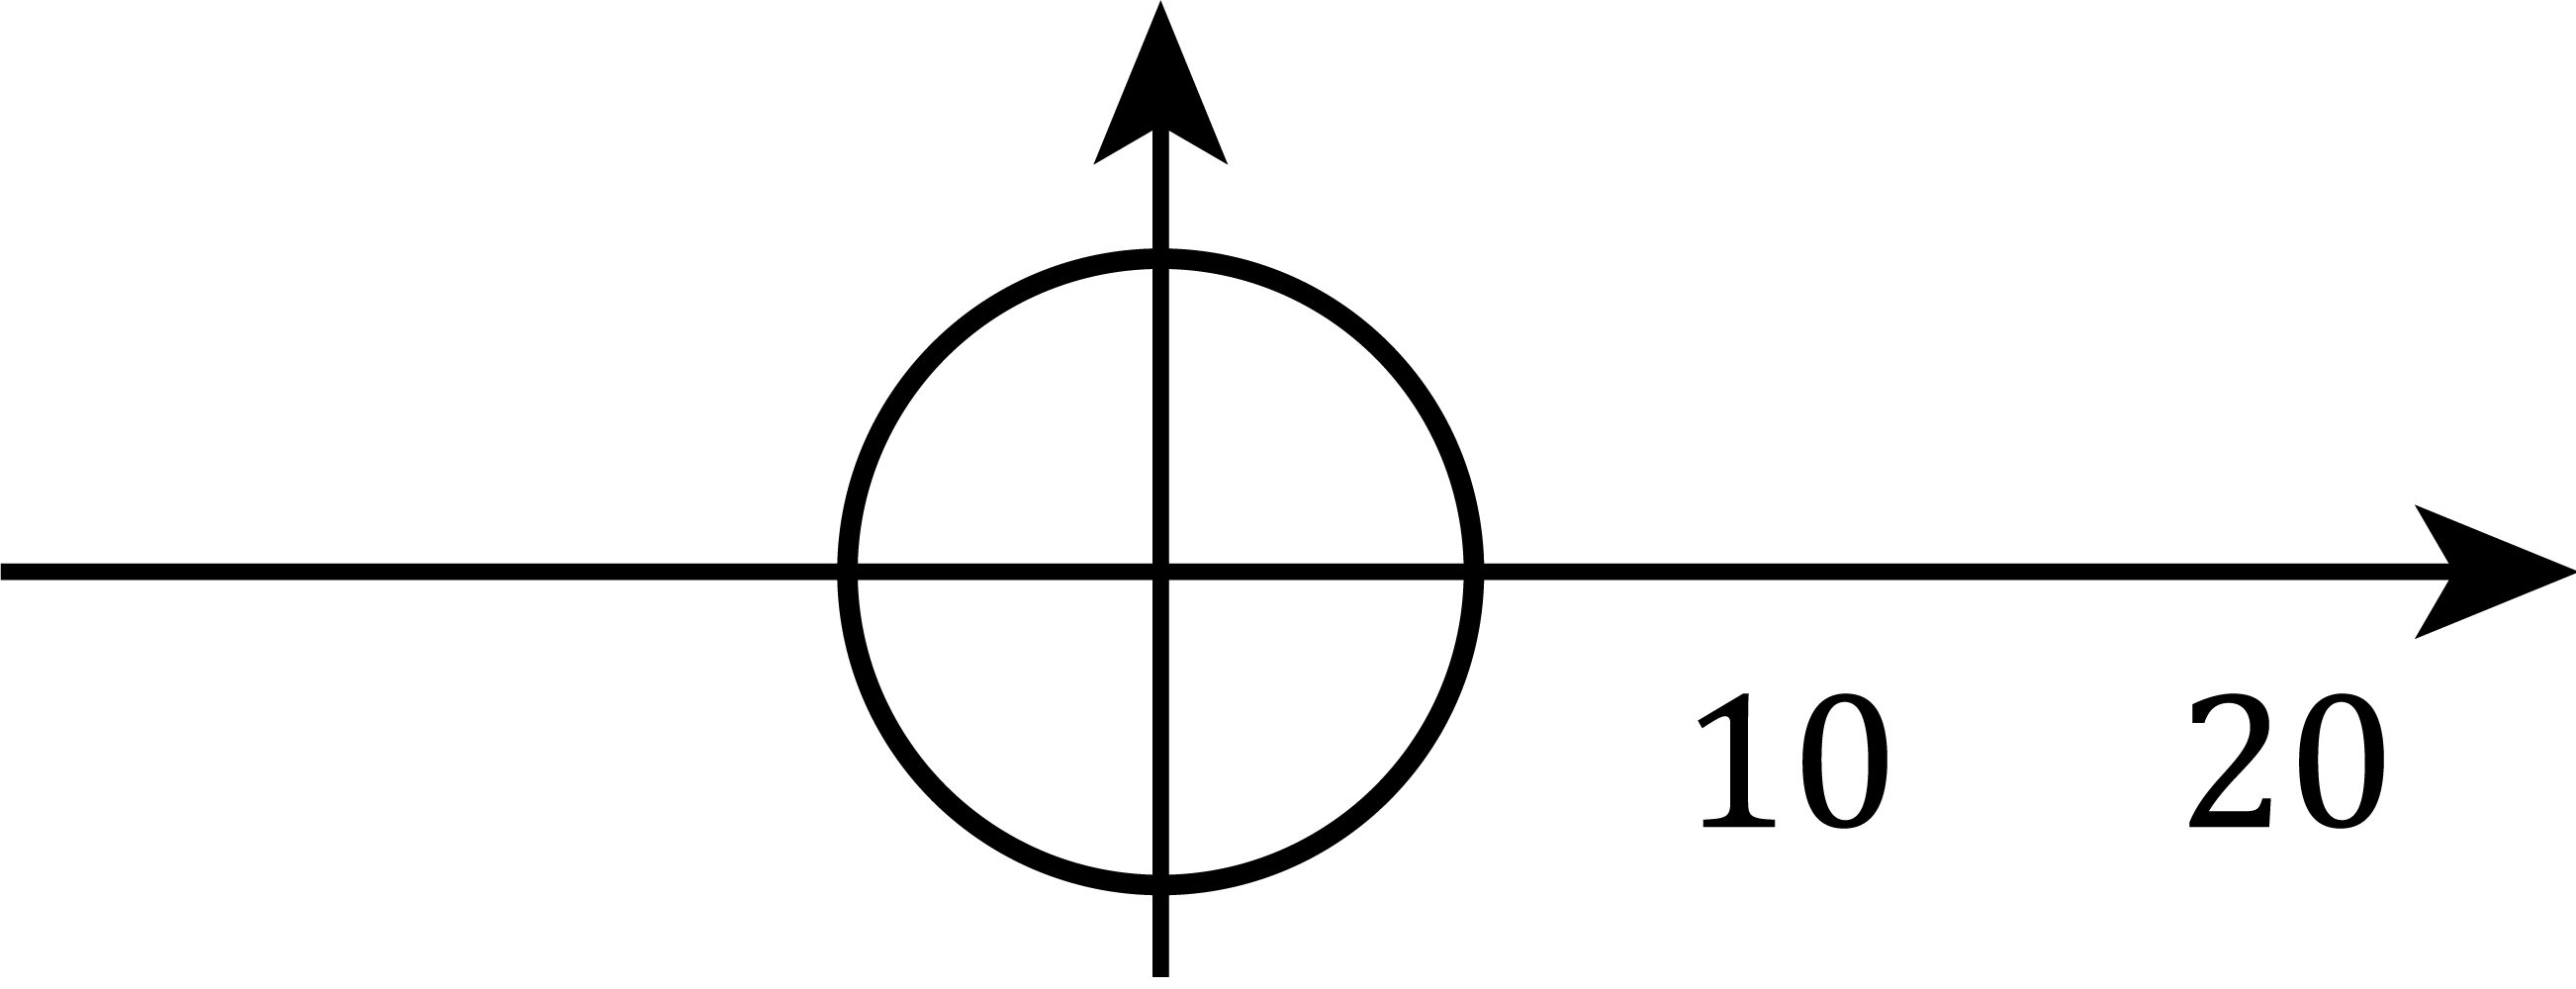
\includegraphics[width=3cm]{10_7}
        \end{figure}
        \[\gamma(t) = a + re^{it} \qq 0 \leq t \leq 2\pi \]
        \[z - a = re^{it} \]
    \end{Example}

    \begin{Example}[2]
        \[hint: \q r e^{i\varphi} = r e^{-i \varphi}  \]
        \[\int_{\gamma(t) = a + e^{it} } \overline{(z - a)}^n dz =  \]
        \[=\int_0^{2\pi} r^n e^{-int} r \cdot i \cdot e^{it}dt =
            i \cdot r^{n + 1}  \int_0^{2\pi} e^{i(1 - n)t}dt =  \]
        \[=ir^{n + 1} \left(\int_0^{2\pi} \cos(1 - n)tdt + i\int_0^{2\pi}
            \sin(1 - n)tdt\right) = \begin{cases}
                0,          & n \neq 1 \\
                2\pi i r^2, & n = 1
            \end{cases}\]
    \end{Example}

    \begin{Utv}
        \[\abs{\int_\gamma f(z)dz} \leq \max_{z \in \gamma} \abs{f(z)} \cdot L(\gamma)\]
    \end{Utv}

    \begin{Proof}
        \[\gamma : [a, b] \to \CC\]
        \[\abs{\int_\gamma f(z)dz} = \abs{\int_a^b f(\gamma(t)) \gamma'(t)dt} \leq
            \int_a^b \us{\leq \displaystyle \max_{z \in \gamma}
                \abs{f(z)}}{\abs{f(\gamma(t))} }\abs{\gamma'(t)}dt \leq \]
        \[\leq \max_{z \in \gamma} \abs{f(z)} \cdot \us{= L(\gamma)}
            {\int_a^b \abs{\gamma'(t)}dt }\]
    \end{Proof}

    \begin{Consequence}
        \[f = \sum_{j = 1}^\infty f_j \text{ --- сх. равн. на } \gamma \]
        Тогда этот ряд можно проинтегрировать почленно
        \[\int_\gamma f(z)dz = \sum_{j = 1}^\infty \int_\gamma f_j(z)dz\]
    \end{Consequence}

    \begin{Proof}
        \[S_N(z) = \sum_{j = 1}^N f_j(z)\]
        \[\int_\gamma f(z)dz = \int_\gamma S_n(z)dz + \int_\gamma (f - S_N)dz\]
        \[\abs{\int_\gamma(f - S_N)dz} \leq \us{\to 0 \text{ (т.к.  }S_N \rightrightarrows f)}{\max_{z \in \gamma}
                \abs{f(z) - S_N(z)} }\cdot \us{const}{L(\gamma)} \]
        \[\int_\gamma f(z)dz = \lim_{N \to \infty}
            \int_\gamma S_N(z)dz = \lim_{N \to \infty}
            \int_\gamma \sum_{j = 1}^N  f_j(z)dz\]
        \[=\lim_{N \to \infty} \sum_{j = 1}^N  \int_\gamma f_j(z)dz =
            \sum^\infty_{j = 1} \int_\gamma f_j(z)dz\]
        \[\int_\gamma \sum^\infty_{j = 1}  f_j(z)dz = \sum_{j = 1}^\infty \int_\gamma f_j(z)dz \]
    \end{Proof}

    \begin{Example}
        \[f(z) = e^{\overline{z}} \]
        \[\gamma(t) = e^{it} \qq 0 \leq t \leq 2\pi \]
        \[e^z = 1 + z + \frac{z^2}{2!} + ... + \frac{z^n}{n!} + ...\]
        \[\overline{D}(0, z) \q \text{ по пр. Вейерштрасса } \qq \sum \frac{z^n}{n!}
            \text{ сх. равн.}\]
        \[\int_{z = e^{it} } e^{\overline{z}}dz = \int_{z = e^{it} }
            \sum_{n = 0}^\infty \frac{\overline{z}^n}{n!}dz  =
            \sum_{n = 0}^\infty \frac{1}{n!} \int_\gamma \overline{z}^{n}dz = 2\pi i  \]
        \[\int_\gamma \overline{z}^ndz = \begin{cases}
                2 \pi i & n = 1    \\
                0       & n \neq 1
            \end{cases}\]
    \end{Example}

    \subsection{Лемма Гурса}

    \begin{Lemma} [Гурса (т. Коши для $\bigtriangleup$)]
        \[\Omega \text{ --- область } \q \Omega \subset \CC\]
        \[f \in H(\Omega \setminus \{p\})\]
        \[f \in C(\Omega)\]
        \begin{figure}[H]
            \centering
            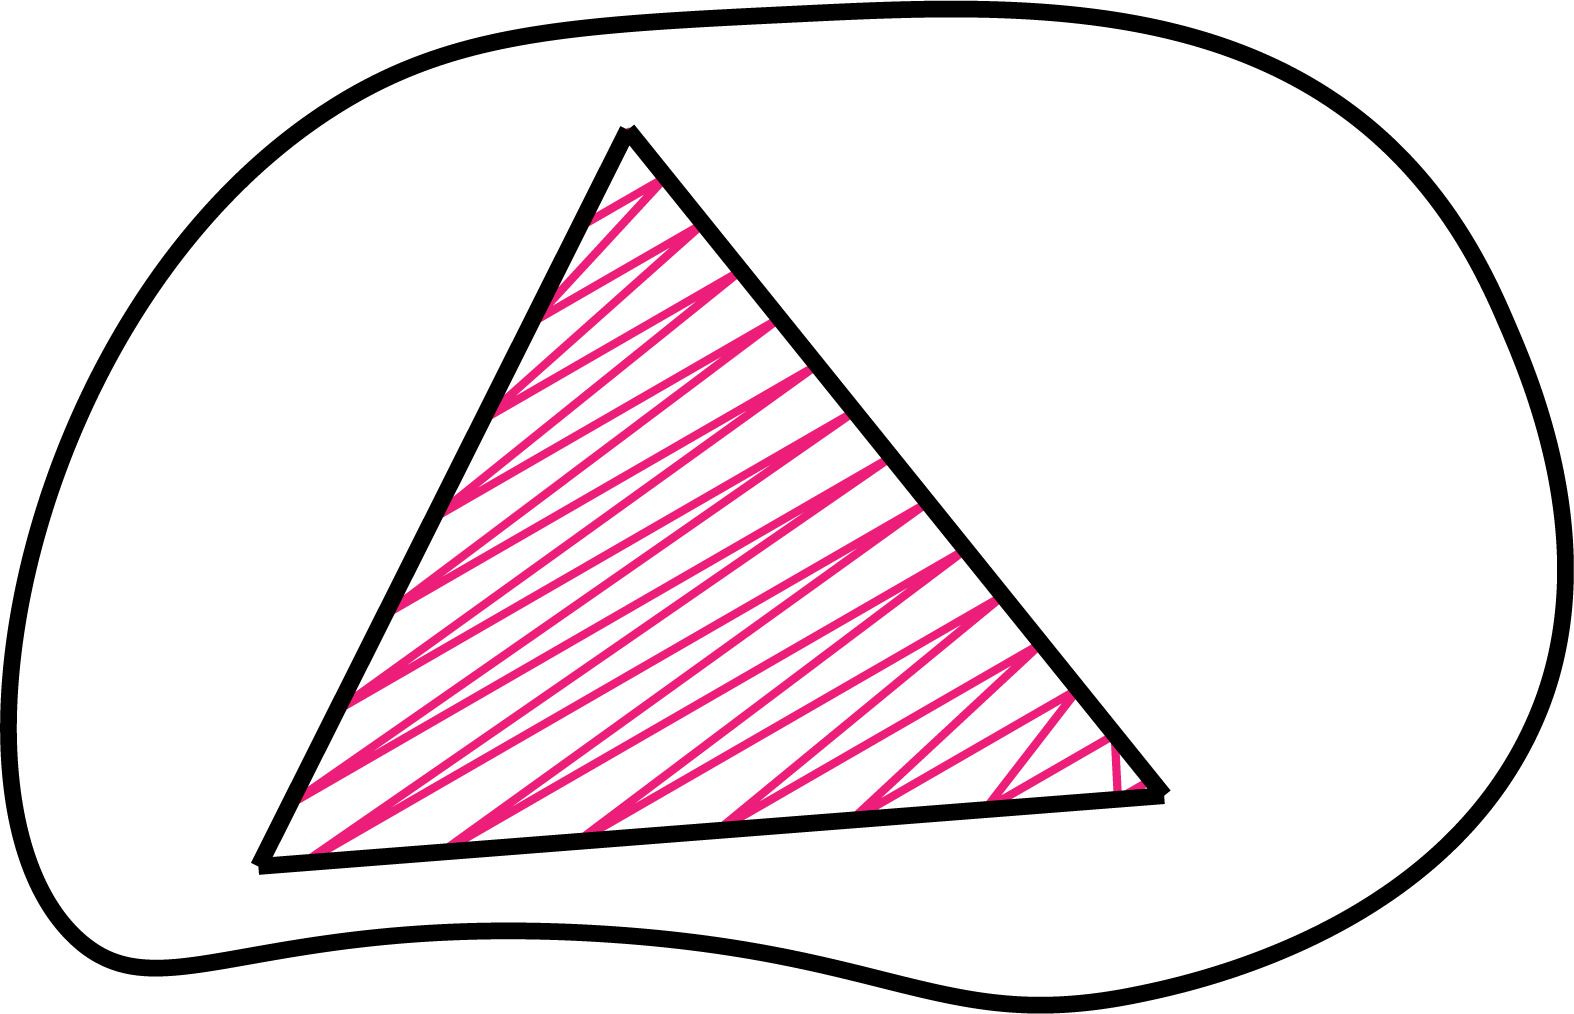
\includegraphics[width=3cm]{10_8}
        \end{figure}
        \[\triangle ABC \subset \Omega \text{ (вместе с внутр.)}\]
        \[\triangle = \triangle ABC\]
        \[\text{Тогда } \qq \int_{\partial \triangle} f(z)dz = 0\]
    \end{Lemma}

    \begin{Proof}
        \[\RNumb{1}) \qq \text{Пусть } P \cancel{\in } \triangle\]
        \begin{figure}[H]
            \centering
            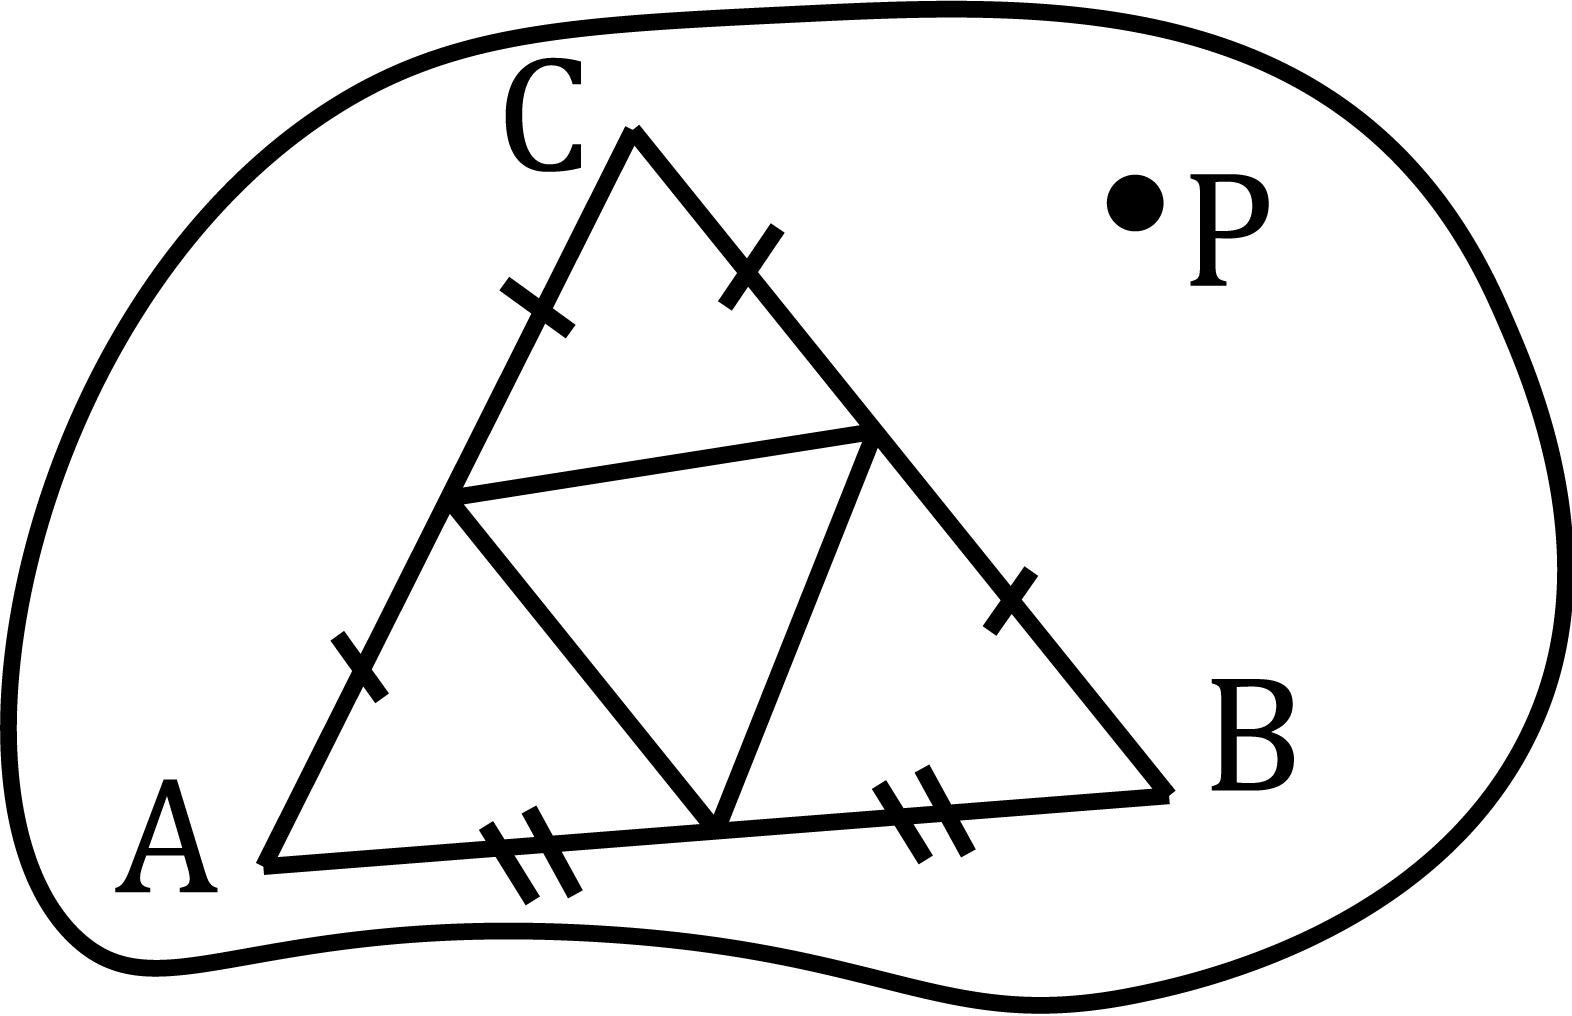
\includegraphics[width=4cm]{10_9}
        \end{figure}
        \[\partial \triangle \text{ --- границы треуг.}\]
        \[J = \int_{\delta \triangle} f(z)dz = \int_{AB} + \int_{BC} + \int_{CA} =
            \sum_{j = 1}^4 \int_{\gamma_j} f(z)dz  \]
        \[\abs{J} \leq \sum_{j = 1}^4 \abs{\int_{\gamma_j} f(z)dz }  \Ra  \text{
                из более мелких $\triangle$ найдется хотя бы один}\]
        \begin{figure}[H]
            \centering
            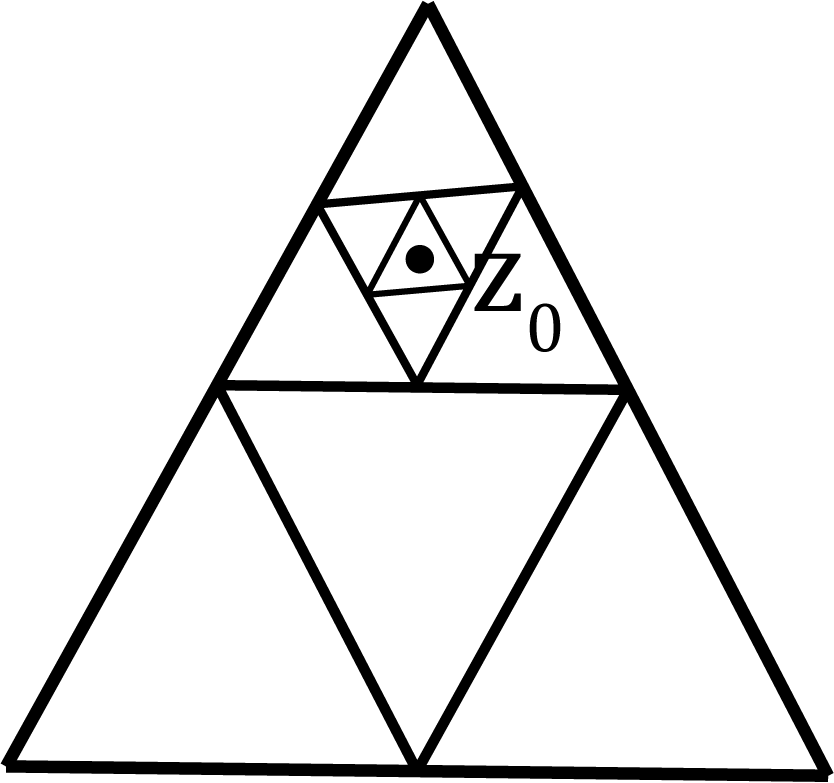
\includegraphics[width=3.5cm]{10_10}
        \end{figure}
        \[\abs{\int_{\partial \trinagle_1}  f(z)dz} \geq \frac{1}{4}\abs{J}\]
        \[\triangle \supset \triangle_1 \supset  \triangle_2 \supset ... \supset
            \triangle_n \supset ...\]
        \[\abs{\int_{\partial \triangle_n} f(z)dz } \geq \frac{1}{4} \abs{
                \int_{\partial \triangle_{n - 1} }f(z)dz } \supset ... \supset \frac{1}{4^n}
            \abs{J}\]
        \[\abs{J} \leq 4^n \int_{\partial \triangle n} f(z)dz \]
        \[L = L(\partial \triangle)\]
        \[L(\partial \triangle_n) = \frac{\triangle}{2^n}\]
        \[\triangle_1 \supset \triangle_2 \supset \triangle_3 ... \supset \triangle_n
            \supset ...\]
        \[\diam \triangle_n \to 0\]
        \[\bigcap_{k = 1}^\infty \triangle_k = \{z_0\} \subset \triangle \subset \Omega \]
        \[f \text{ --- диф-ма в т. } z_0 \Ra\]
        \[\lim_{z \to  z_0} \frac{f(z) - f(z_0)}{z - z_0}  = f'(z_0)\]
        \[\forall \mathcal{E} > 0 \q \exists  \delta : \abs{z - z_0} < \delta \Ra\]
        \[\abs{f(z) - f(z_0) - f'(z_0)(z - z_0)} < \mathcal{E}[z - z_0]\]
        \[\text{т.к. } \text{diam}(\triangle_n) \to  0 \Ra \exists  n_0 : \forall  n >
            n_0\]
        \[\forall z \in \overline{\triangle_n} \qq
            \abs{f(z) - f(z_0) - f'(z_0)(z - z_0)} < \mathcal{E}\abs{z - z_0}\]
        \[\int_{\partial \triangle_n} f(z)dz = \int_{\partial \triangle_n}
            (f(z) - f(z_0) - f'(z_0)(z - z_0))dz\]
        \[\text{т.к. } \int_{\gamma} (az + b)dz = \int_{\gamma} d(\frac{az^2}{2} + bz)  \]
        %Бум! стерли! TODO
        ~Кажется, тут не хватает кусочка~
        \[\abs{\int_{\partial \triangle_n} f(z)dz} =\abs{ \int_{\partial \triangle_n}
            (f(z) - f(z_0) - f'(z_0)(z - z_0))dz} \leq \]
        \[\leq \max_{\delta \triangle_n} \abs{f(z) - f(z_0) - f'(z_0)(z - z_0)} \cdot
            L(\partial \triangle_n) < \mathcal{E} \cdot L(\partial \triangle_n)^2 =
            \mathcal{E} (\frac{L}{2^n})^2\]
        \[\abs{J} \leq 4^n \abs{\int_{\partial \triangle_n} f(z) dz} <
            4^n \mathcal{E} \frac{L^2}{4^n}  = \mathcal{E} L^2 \qq \forall \mathcal{E} > 0\]
        \[\Ra \abs{J} = 0\text{, т.е } \int_{\triangle} f(z)dz = 0 \]

        \[\RNumb{2}) \text{ если } p \in \text{ одна из вершин } \qq \text{напр. } p = A\]
        \begin{figure}[H]
            \centering
            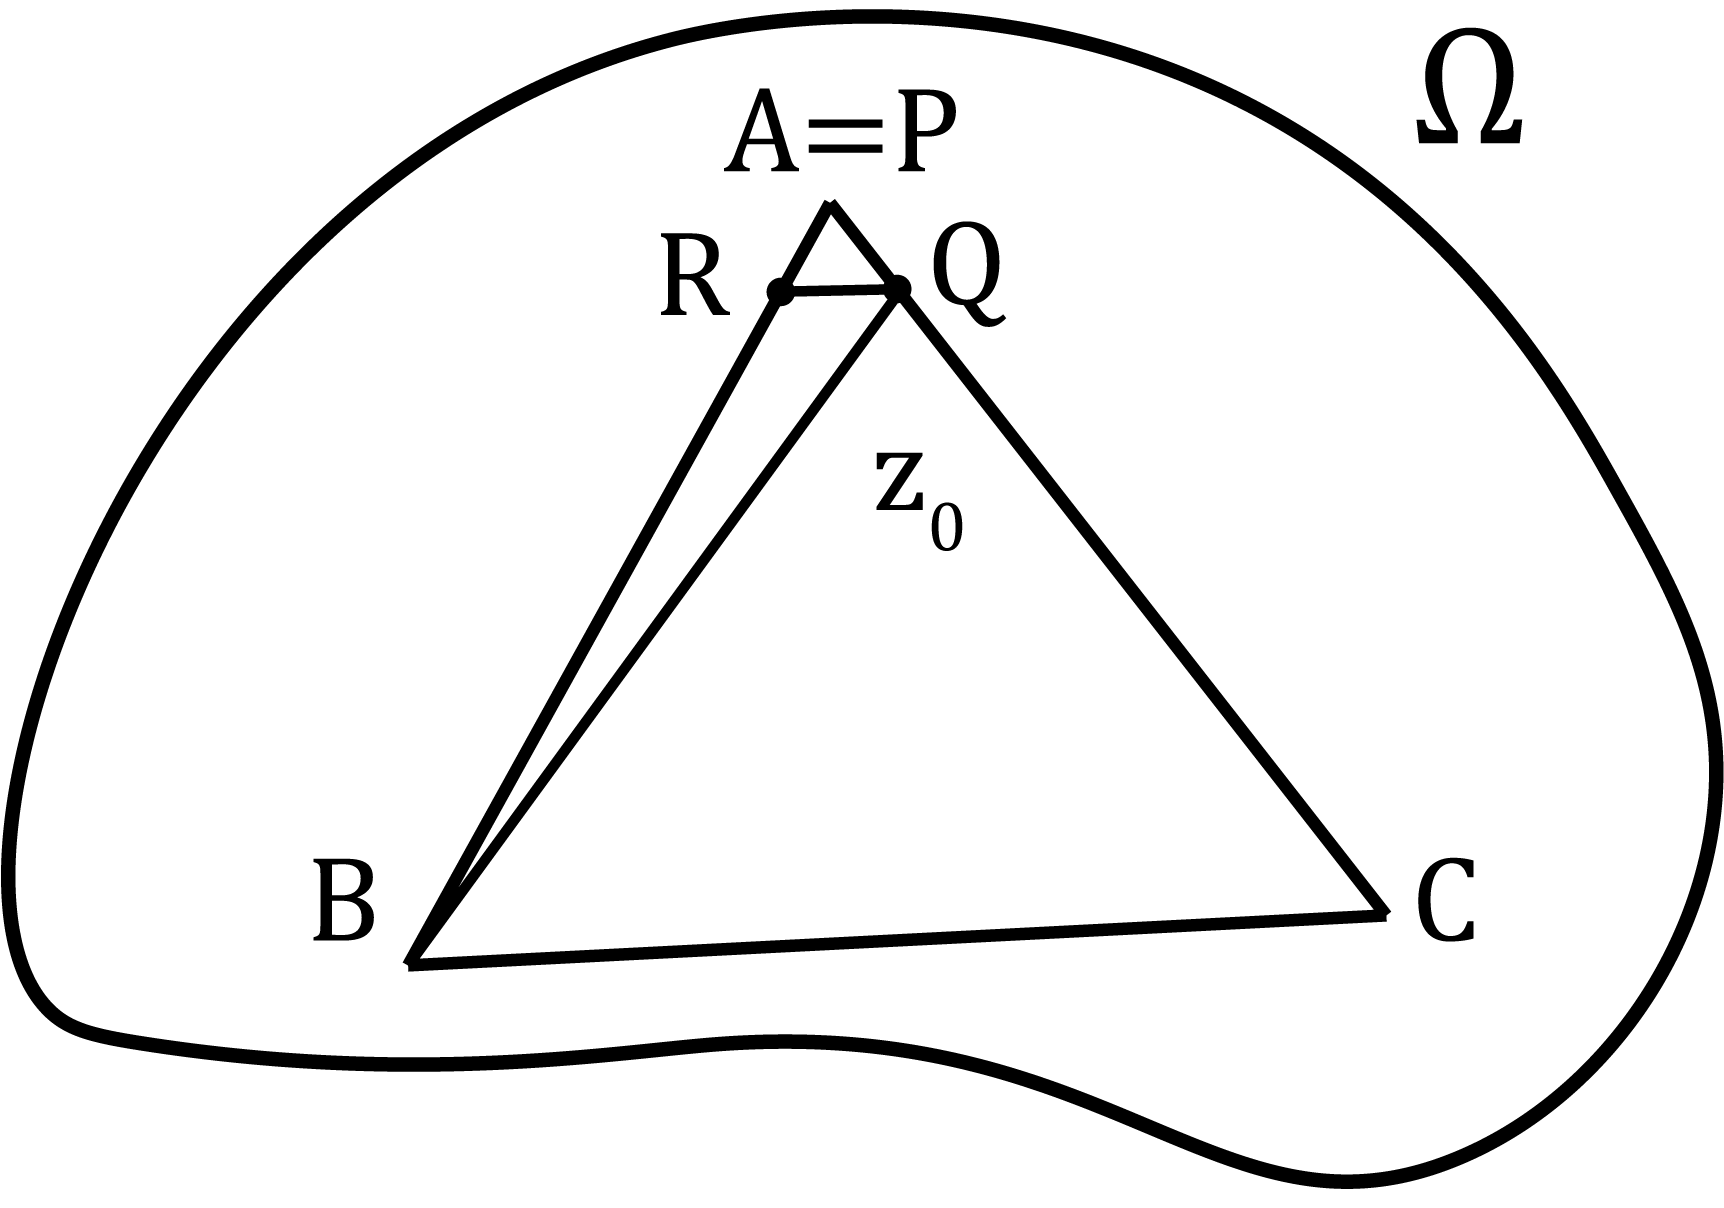
\includegraphics[width=6cm]{10_11}
        \end{figure}
        \[\text{по п. } \RNumb{1} \qq \int_{\triangle BQR} f = \int_{BCQ} f = 0  \]
        \[\abs{\int_{\triangle PQA} f(z)dz} \leq M \cdot L(\triangle RQA) \]
        \[f \text{ - непр. на комп. } \Ra \abs{f} \leq M < \infty\]
        \[\forall  \mathcal{E} > 0 \q \exists  R, Q :\q  L(\triangle RQA) < \mathcal{E}\]
        \begin{figure}[H]
            \centering
            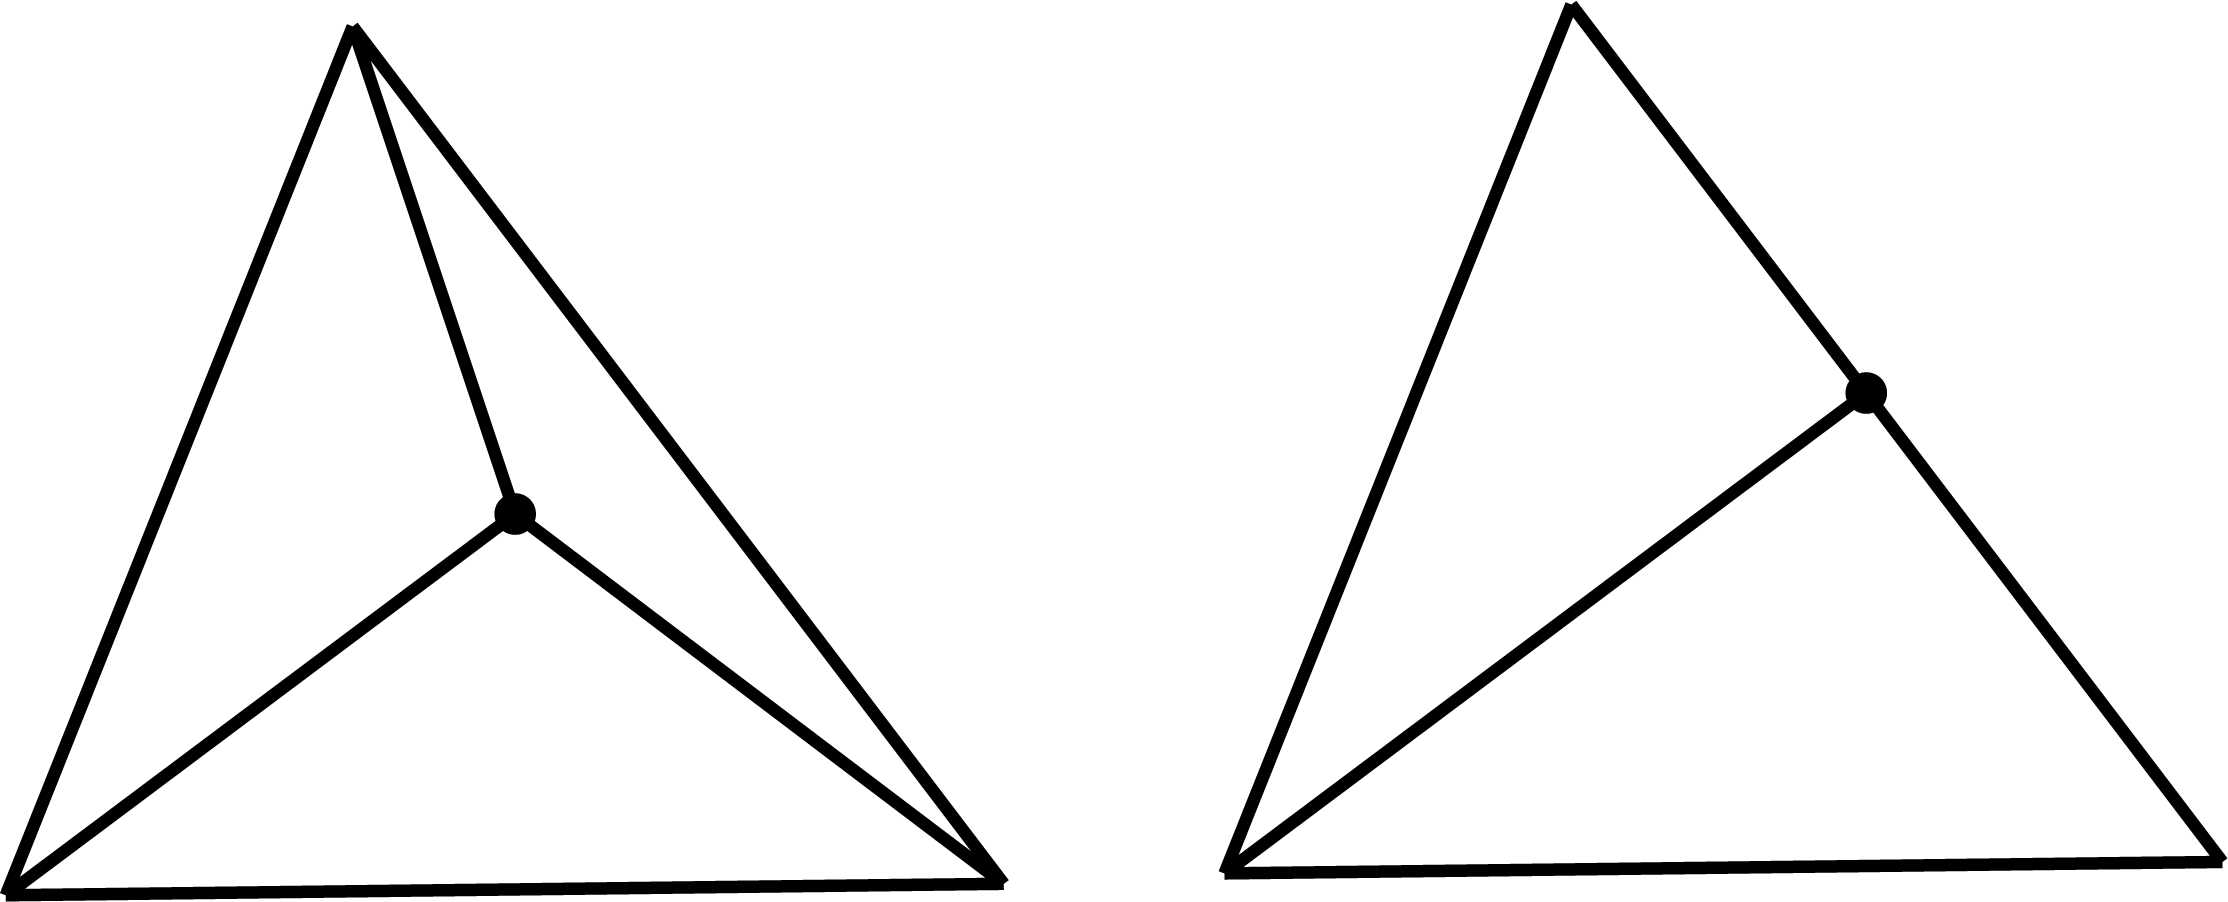
\includegraphics[width=5cm]{10_12}
        \end{figure}
    \end{Proof}
\end{lect}
\end{document}
